\documentclass[a4paper]{article}
% definitions
\def\D{\partial}
\def\a{\alpha}
\def\dd{\displaystyle}
\def\ke{{k- \varepsilon}}
\def\e{\varepsilon}
\def\12{{\frac{1}{2}}}
\def\ub{\bar{u}}
\def\vb{\bar{v}}
\def\pb{\bar{p}}
\def\vij{\overline{v'_iv'_j}}
\def\vik{\overline{v'_iv'_k}}
\def\vjk{\overline{v'_jv'_k}}
\def\uv{\overline{v'_1v'_2}}
\def\vw{\overline{v'_2v'_3}}
\def\uw{\overline{v'_1v'_3}}
\def\uu{\overline{v_1^{\prime 2}}}
\def\vv{\overline{v_2^{\prime 2}}}
\def\ww{\overline{v_3^{\prime 2}}}
\def\karm{von  K\'arm\'an }
\def\solidline{{$\textcolor{blue}{\overline{\hskip 0.5cm}}\ $}}
\def\dashedline{{$\textcolor{red}{\overline{\hskip 0.1cm}\ \overline{\hskip 0.1cm}\ \overline{\hskip 0.1cm}\ }$}}
\def\dashdottedline{$\overline{\hskip 0.1cm}\ \overline{\hskip 0.03cm}\ \overline{\hskip 0.1cm}\ $}
\def\dottedline{$\overline{\hskip 0.04cm}\ \overline{\hskip 0.04cm}\ \overline{\hskip 0.04cm}\ $}

% packages
\usepackage{color}
\usepackage{listings}
\lstset{language=C++,frame=lines}
\lstset{language=Gnuplot,frame=lines}
\lstset{language=Matlab,frame=lines}
\lstset{language=Fortran,frame=lines}
% \usepackage{subfigure} % <--- RIMOSSO: va in conflitto con subcaption
\usepackage{graphicx,psfrag}
\usepackage{amsmath}
\usepackage{amsfonts}
\usepackage{latexsym}
\usepackage{amssymb}
\usepackage{pst-all}
\usepackage{float}
\usepackage[colorlinks=true,linkcolor=blue,anchorcolor=blue,urlcolor=blue,citecolor=blue]{hyperref}
\usepackage{multicol}
\usepackage{nomencl}
\usepackage{makecell}
\usepackage{array}
\usepackage{booktabs}
\usepackage{xcolor}
\usepackage{subcaption} % <--- MANTENUTO (versione moderna per le subfigure)
\usepackage[nottoc]{tocbibind}

\definecolor{f_kw}{RGB}{0,0,255}   % Blu per parole chiave (f_kw)
\definecolor{f_cm}{RGB}{34,139,34} % Verde per commenti (f_cm)
\definecolor{f_st}{RGB}{163,21,21} % Rosso scuro per stringhe (f_st)
\definecolor{foambackground}{RGB}{250,250,250}

\lstdefinelanguage{OpenFOAM}{
	morekeywords={FoamFile,version,format,class,object,application,startFrom,startTime,stopAt,endTime,deltaT,writeControl,writeInterval,purgeWrite,writeFormat,writePrecision,writeCompression,timeFormat,timePrecision,runTimeModifiable,functions,type,libs,patches,coordinateSystem,origin,rotation,e1,e2,rho,rhoInf,CofR,log,calcCoeff,result,writeControl},
	sensitive=true,
	morecomment=[l]{//},
	morecomment=[s]{/*}{*/},
	morestring=[b]"
}

% --- 3. STILI PERSONALIZZATI ---
\lstdefinestyle{compactBase}{
	basicstyle=\ttfamily\scriptsize,
	breaklines=true,
	breakatwhitespace=true,
	frame=single,
	showstringspaces=false,
	xleftmargin=5pt,
	xrightmargin=5pt,
	tabsize=2,
	lineskip=-1pt,
	commentstyle=\color{f_cm},
	keywordstyle=\color{f_kw}\bfseries,
	stringstyle=\color{f_st}
}

\lstdefinestyle{ofStyle}{
	style=compactBase,
	language=OpenFOAM
}

\lstdefinestyle{bashStyle}{
	style=compactBase,
	language=bash
}

\pagestyle{myheadings}

\renewcommand{\subsectionmark}[1]{\markright{\thesubsection. #1}}
\renewcommand{\sectionmark}[1]{\markright{\thesection. #1}}

\begin{document}
	
	\setcounter{page}{1}
	% --- NUOVA COPERTINA ---
	\begin{titlepage}
		\begin{center}
			\vspace*{-1.5cm}
			{\large \textbf{ALMA MATER STUDIORUM -- UNIVERSITY OF BOLOGNA}} \\[0.2cm]
			\rule{\textwidth}{0.4pt} \\[0.5cm] 
			
			{\Large \textbf{FORL\`I CAMPUS}} \\[0.5cm]
			{\large \textbf{Department of Industrial Engineering -- DIN}} \\[0.5cm]
			{\large Degree Programme in }\\
			{\large \textbf{AEROSPACE ENGINEERING}}\\[5cm] 
			{\huge \textbf{OpenFOAM Formula SAE Case Implementation}} \\[1cm]
			{\Large \textbf{INTERNSHIP REPORT}}
		\end{center}
		
		\vfill 
		
		\begin{minipage}[t]{0.47\textwidth}
			{\textbf{Academic supervisor:}}\\[0.2cm]
			{Prof. Guglielmo Minelli}
		\end{minipage}\hfill
		\begin{minipage}[t]{0.47\textwidth}\raggedleft
			{\textbf{Candidate:}}\\[0.2cm]
			{Jacopo Turrini}
		\end{minipage}
	\end{titlepage}
	% --- FINE COPERTINA ---
	
	\tableofcontents
	
	\newpage
	\listoffigures
	\newpage
	\listoftables
	\newpage
	
	\section*{Abstract}
	As part of my bachelor's degree requirements, I completed an internship in Computational Fluid Dynamics (CFD) under the supervision of Prof. Guglielmo Minelli.
	During the initial phase of this project, I focused on mastering the foundational principles of OpenFOAM, successfully executing standard tutorials such as "motorBikeSteady".
	Upon gaining proficiency in OpenFOAM dictionaries, directory structures, and the functional role of individual configuration files, I proceeded to develop the simulation case for "Visione": the prototype engineered by UniBO Motorsport for the current season's Formula Student Electric (EV) category.
	I evaluated various turbulence models for my RANS simulations; while the Spalart-Allmaras model initially yielded satisfactory results, I subsequently identified inconsistencies regarding characteristic vortices when compared to the $k-\omega$ SST model typically employed by UniBO Motorsport for aerodynamic development.
	\newpage
	
	\section{Introduction}
	This report documents the methodology and findings of my research into the fundamentals of CFD.
	OpenFOAM serves as an exemplary educational platform due to its open-source framework: it requires the engineer to explicitly define boundary conditions, select appropriate turbulence models, and differentiate between first and second-order numerical schemes, fostering a comprehensive understanding of the discipline.
	Furthermore, OpenFOAM is freely licensed, enabling users to perform sophisticated simulations without commercial constraints.
	By developing this case, I primarily aim to broaden my technical expertise.
	However, this work is also intended to provide tangible benefits to UniBO Motorsport (UBM): the ultimate objective is to implement a parametric study on aerodynamic "flags" (winglets) and to establish a robust workflow allowing UBM to leverage CINECA high-performance computing resources for OpenFOAM aerodynamic simulations. 
	
	Using the knowledge I found in a teammate's thesis work \cite{Bellucci} and across multiple forums and sites (\cite{OpenFoamDoc}, \cite{SimScaleFS}, \cite{leap}, \cite{SimScaleFS}, \cite{CFDOnline}), I managed to implement a working case for the 2026 prototype of the UniBO Motorsport team. On these same sites and forums, I found out that the aerodynamic appendages we refer to as "flags" within the team are usually known as guide-vanes, a much more generic term. Because Formula SAE (and motorsport in general) is highly competitive, it is clear that no team is particularly keen to publish its own research, resulting in little to no public documentation on the topic. The upcoming thesis work I will develop will focus on understanding what these wings do, as well as maximizing their performance.
	
	
	\section{Theory}
	Computational Fluid Dynamics is a powerful engineering methodology that enables the analysis of aerodynamic performance relative to geometry through the numerical solution of mathematical equations.
	While solving the Navier-Stokes equations across a continuous domain is ideal, obtaining exact analytical solutions for complex geometries is computationally prohibitive.
	\[ \begin{cases}
		{\frac{\partial{\rho}}{\partial{t}}}+{\frac{\partial{\rho u_{i}}}{\partial{x_{i}}}}=0\\
		\rho\  \frac{Du_{i}}{Dt}= \rho f_{i} - \frac{\partial p}{\partial x_{i}} + (\lambda+ \mu)\frac{\partial }{\partial x_{i}}\left( \frac{\partial u_{k}}{\partial x_{k}}\right)+ \mu \frac{\partial^{2} u_{i}}{\partial x_{j} \partial x_{j}}\\
		\rho c_{V} \frac{D\theta}{Dt}=-\frac{\partial{u_{i}}}{\partial{x_{i}}} \left[\theta  \left(\frac{\partial{p}}{\partial{\theta}}\right)_{v}\right]+\sigma_{ij} \frac{\partial{u_{i}}}{\partial{x_{j}}}- \frac{\partial{q_{i}}}{\partial{x_{i}}}+ \rho Q
	\end{cases} \]
	To facilitate CFD simulations, several standard assumptions and simplifications are introduced:
	\begin{itemize}
		\item The simulation is steady-state, neglecting all time-dependent terms.
		\item Based on the team's nominal testing velocity of 15.56 m/s and a maximum velocity not exceeding 34 m/s, the flow is modeled as incompressible ($\rho = \text{constant}$ and $\frac{\partial u_i}{\partial{x_i}}=0$).
		\item The energy conservation equation is omitted from the governing system.
	\end{itemize}
	The Navier-Stokes equations are simplified as follows:
	\[ \begin{cases}
		{\frac{\partial{ u_{i}}}{\partial{x_{i}}}}=0\\
		\rho\ u_j \frac{\partial u_{i}}{\partial x_j}= \rho f_{i} - \frac{\partial p}{\partial x_{i}}+ \mu \frac{\partial^{2} u_{i}}{\partial x_{j} \partial x_{j}}\\
	\end{cases}\implies \begin{cases}
		{\frac{\partial{ u_{i}}}{\partial{x_{i}}}}=0\\
		u_j \frac{\partial u_{i}}{\partial x_j}=  f_{i} - \frac{1}{\rho}\frac{\partial p}{\partial x_{i}}+ \nu \frac{\partial^{2} u_{i}}{\partial x_{j} \partial x_{j}}\\
	\end{cases} \]
	Boundary conditions must be rigorously defined for these differential equations:
	\begin{itemize}
		\item $u_i|_\infty = \vec U_\infty$ (Freestream velocity)
		\item $u_i|_{wall} = 0$ (No-slip condition)
		\item A reference pressure datum must be established.
		\item Accurate modeling of turbulent viscosity is essential, as this represents the primary point of divergence between various turbulence models.
	\end{itemize}
	\begin{enumerate}
		\item \textbf{Spalart-Allmaras}: This model approximates turbulence using a single-equation transport model for a modified viscosity term, $\tilde \nu$.
		Originally developed by Boeing for external aerodynamic flows, it exhibits linear behavior near walls, contributing to high numerical stability.
		While $\nu_t$ represents the turbulent viscosity, $\tilde \nu_t$ is a computational intermediate without direct physical meaning.
		\item \textbf{$k-\omega$ Shear Stress Transport (SST)}: A hybrid model that leverages the strengths of $k-\omega$ (near-wall accuracy) and $k-\epsilon$ (freestream stability).
		$k$ (Turbulent Kinetic Energy) represents turbulence intensity, while $\omega$ (Specific Dissipation Rate) defines the scale of energy dissipation.
		The SST formulation constraints turbulent viscosity to prevent the over-prediction of flow attachment under adverse pressure gradients.
		\[u_j\frac{\partial k}{\partial x_j}= \frac{\partial}{\partial x_j}\left[(\nu+ \sigma_k\nu_t)\frac{\partial k}{\partial x_j}\right]+ P_k - \beta ^* \omega k\]
		\[u_j \frac{\partial \omega}{\partial x_j} = \frac{\partial}{\partial x_j} \left[ \left( \nu + \sigma_{\omega} \nu_t \right) \frac{\partial \omega}{\partial x_j} \right] + \gamma \frac{P_k}{\nu_t} - \beta \omega^2 + 2 (1 - F_1) \sigma_{\omega 2} \frac{1}{\omega} \frac{\partial k}{\partial x_j} \frac{\partial \omega}{\partial x_j}\]
	\end{enumerate}
	As these calculations cannot be performed across a continuous domain, the volume must be discretized into a finite number of cells (a mesh).
	Mesh quality profoundly influences results and must adhere to several criteria:
	\begin{itemize}
		\item \textbf{$y^+$}: A critical non-dimensional parameter representing the distance from the wall to the first cell node.
		$$Re= \frac{Lu}{\nu}\to y^+= \frac{y_1u_\tau}{\nu}$$
		where $u_\tau$ is the friction velocity and $y_1$ is the absolute distance from the wall.
		For $y^+\leq 1$, the mesh is sufficient to resolve the viscous sublayer;
		for $y^+\geq 30$, the boundary layer is modeled using logarithmic wall functions.
		The range $1 < y^+ < 30$ (the buffer zone) should be avoided to maintain accuracy.
		\item \textbf{Cell Aspect Ratio}: Defines cell proportions; these must remain within specified limits to ensure numerical stability.
		\item \textbf{Layer Growth Ratio}: Governs the expansion rate between consecutive mesh layers.
	\end{itemize}
	
	In mastering the software and developing these skills, I referenced extensive online documentation, tutorials from SimScale and OpenFOAM.com, and community forums such as CFD Online and Reddit.
	I also consulted Prof. Guglielmo Minelli for strategic guidance regarding project direction.
	\subsection{Methodology}
	Acquiring new skills must certainly begin with the theoretical foundations to understand what is going to be done, but it also relies on making and correcting mistakes, trying solutions that others have found, and adapting them to one's own case. I decided to start by learning the basics of computational fluid dynamics (CFD). Then, I attempted to master some tutorials of interest (like \texttt{motorBikeSteady}) and started making some tweaks to them, trying to get closer and closer to the final goal.
	
	\subsection{CFD Setup}
	Initial attempts to adapt existing meshes to OpenFOAM proved problematic; while Fluent predicted attached flow, OpenFOAM exhibited numerical instabilities and predicted premature flow separation.
	The updated model established by Marco Bellucci \cite{Bellucci} incorporates:
	\begin{itemize}
		\item \textbf{Shell Type and Size:} The model utilizes a combination of first-order triangular and quadrilateral shell elements.
		Global resolution is governed by the defined Minimum and Maximum Shell Size.
		\item \textbf{Growth Ratio:} This factor is maintained between 1.0 and 1.3 to minimize size gradients between adjacent cells and ensure smooth transitions.
		\item \textbf{Distortion Angle:} Restricted to a maximum of 15$^\circ$ to provide adequate discretization of surface curvature.
		\item \textbf{Feature-Specific Refinement:}
		\begin{itemize}
			\item \textbf{Leading Edges (LE):} Meshed with an anisotropic structure, refined in the streamwise direction to capture steep pressure gradients.
			\item \textbf{Trailing Edges (TE) and Fillets:} Discretized employing a structured approach with at least three rows of quadrilateral elements.
			\item \textbf{Sharp Edges:} Local refinement is applied to improve resolution in high-criticality zones.
		\end{itemize}
	\end{itemize}
	
	\begin{itemize}
		\item \textbf{Layer Setup:} Defined by the First Layer Height (FLH), Layer Growth Ratio (LGR), and the Number of Layers (NL).
		\item \textbf{Growth Ratio:} Maintained between 1.1 and 1.2 to ensure adequate discretization across the boundary layer region.
		\item \textbf{Target Resolution:} The FLH is determined by the selected wall treatment \cite{SimScaleFS}:
		\begin{itemize}
			\item \textit{Low-$y^{+}$ approach:} $y^{+} \approx 1$ for wall-resolved simulations.
			\item \textit{High-$y^{+}$ approach:} $y^{+} \geq 30$ for wall-function simulations within the log-law region.
		\end{itemize}
		\item \textbf{Quality Control:} A compression (squeezing) factor is applied to layers in narrow or complex geometric regions to prevent cell intersection and maintain mesh quality.
	\end{itemize}
	
	\begin{figure}[H]
		\begin{subfigure}{0.48\linewidth}
			\centering
			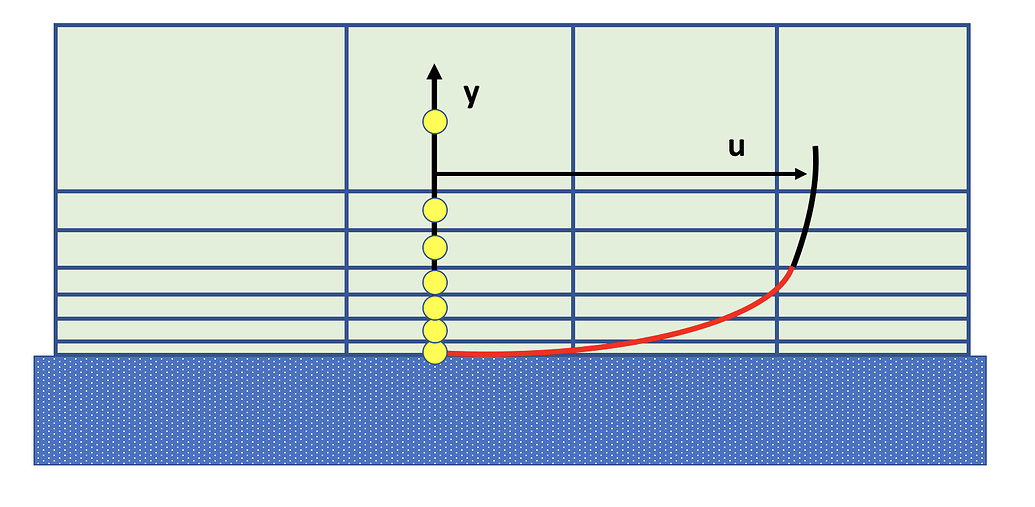
\includegraphics[width=\linewidth]{y+_1}
		\end{subfigure}
		\hfill
		\begin{subfigure}{0.48\linewidth}
			\centering
			\includegraphics[width=\linewidth]{y+_30}
		\end{subfigure}
		\caption{Left: $y^+ < 1$, where mesh density is sufficient to capture all turbulence scales near the wall.
			Right: $y^+ > 30$, where the smallest turbulence scales are approximated via wall functions.
			The latter approach is significantly more computationally efficient, albeit less precise.}
		\label{fig:yplus_comp}
	\end{figure}
	
	\subsubsection*{Volume Mesh and Refinement Strategies}
	\begin{itemize}
		\item \textbf{Volume Filling:} Hexahedral cells populate the remaining domain volume, with dimensions determined by user-defined limits and local refinement constraints.
		\item \textbf{Size Boxes:} These 3D zones impose surface and volume size constraints.
		They are strategically positioned aft of the vehicle to capture wake structures and forward to accurately resolve the pressure signal.
	\end{itemize}
	The meshing parameters used by the team evolved and improved throughout the year, culminating in values that were first developed by Marco Bellucci \cite{Bellucci} and slightly tweaked to ensure the correct discretization on every surface of the new car (Table \ref{tab:full_car_meshing}). 
	Table \ref{tab:boundary_conditions} lists all the boundary conditions that I used for this case.
	
	\begin{table}[H]
		\centering
		\renewcommand{\arraystretch}{1.3}
		\caption{Full car model meshing parameters \cite{Bellucci}}
		\label{tab:full_car_meshing}
		\resizebox{\linewidth}{!}{
			\begin{tabular}{l p{8cm}}
				\toprule
				\textbf{Meshing Parameter} & \textbf{Value / Description} \\
				\midrule
				Maximum Surface Shell Size & 6 mm (Coarse size, selected from the grid convergence study). \\
				Shell Cells Type & Mixed type, alternating between triangular and quadrilateral cells. \\
				Shell Cells Order & First order (nodes are placed only at the vertices of the edges). \\
				Maximum Distortion Angle & 15 degrees. \\
				Trailing Edges (TE) \& Fillets & Meshed in a structured way with a minimum of three rows of quadrilateral elements. \\
				Leading Edges (LE) & Meshed with an anisotropic structure, more refined along the streamwise direction. \\
				Inflation Layers Approach & High-$y^+$ approach (target $y^+ \approx 30$) chosen for the full car models. \\
				First Layer Height (FLH) & Computed automatically per PID to place the first cell centroid inside the Overlap Region (OL) of the turbulent boundary layer. \\
				Layer Growth Ratio (LGR) & Kept between 1.1 and 1.2. \\
				Number of Layers (NL) & Computed automatically per component (PID) based on its reference length, the target $y^+$, and the chosen LGR. \\
				Layer Cell Type & Pentahedral or hexahedral extruded cells. \\
				Volume Mesh Cell Type & Hexahedral cells. \\
				\bottomrule
			\end{tabular}
		}
	\end{table}
	
	\begin{table}[H]
		\centering
		\renewcommand{\arraystretch}{1.3}
		\caption{Boundary Conditions by Patch and Field \cite{OpenFoamDoc}\cite{Welahetti}}
		\label{tab:boundary_conditions}
		\resizebox{\linewidth}{!}{
			\begin{tabular}{lccccc}
				\toprule
				\textbf{Patch} & \textbf{U} & \textbf{p} & \textbf{k} & \textbf{$\omega$} & \textbf{$\nu_t$ (nut)} \\ 
				\midrule
				\textbf{Inlet} & {fixedValue} & {freestreamPressure} & {fixedValue} & {fixedValue} & {calculated} \\ 
				\textbf{Outlet} & {zeroGradient} & {fixedValue} & {inletOutlet} & {inletOutlet} & {calculated} \\ 
				\textbf{Symmetry} & {symmetry} & {symmetry} & {symmetry} & {symmetry} & {symmetry} \\ 
				\textbf{Road} & {fixedValue} & {zeroGradient} & {kqRWallFunction} & {omegaWallFunction} & {nutkRoughWallFunction} \\ 
				\textbf{Wheels} & {rotatingWallVelocity} & {zeroGradient} & {kqRWallFunction} & {omegaWallFunction} & {nutUSpaldingWallFunction} \\ 
				\textbf{Car Body} & {noSlip} & {zeroGradient} & {kqRWallFunction} & {omegaWallFunction} & {nutUSpaldingWallFunction} \\ 
				\textbf{Vent Out Diff} & {fixedValue} & {zeroGradient} & {kqRWallFunction} & {omegaWallFunction} & {calculated} \\ 
				\bottomrule
			\end{tabular}
		}
	\end{table}
	
	\subsection{Experimental Setup}
	Validation against empirical data remains a primary challenge, as results can only be fully verified after the physical vehicle is manufactured.
	The proposed validation strategy involves applying the current meshing parameters to last year's car and utilizing tufts combined with an on-board camera to correlate flow separation behavior between the physical car and the CFD model.
	The visual comparison of $y^+$ configurations (Figure \ref{fig:yplus_comp}) highlights the critical trade-off between near-wall resolution and computational efficiency. To validate these CFD assumptions, qualitative on-track tuft testing (Figure \ref{fig:track_testing}) was employed, establishing a physical baseline for flow attachment on the rear elements and confirming the reliability of the aerodynamic model.
	
	\begin{figure}[H]
		\centering
		\includegraphics[width=0.4\linewidth]{"Immagine 2026-03-28 083910"}
		\caption{On-track footage: the tuft behavior indicates minimal flow separation, suggesting that the model is either accurately predicting or slightly under-estimating flow attachment.}
		\label{fig:track_testing}
	\end{figure}
	
	\section{Results}
	Following the successful mastery of the OpenFOAM workflow via the \texttt{motorBikeSteady} tutorial, I initiated the development of vehicle-specific simulation cases.
	The Spalart-Allmaras turbulence model was initially selected due to its computational efficiency and the straightforward relationship between \texttt{nut} and \texttt{nuTilda}.
	
	\begin{figure}[H]
		\begin{subfigure}{\linewidth}
			\centering
			\includegraphics[width=\linewidth]{"comparison"}
		\end{subfigure}
		\par\vspace{0.5cm}
		\begin{subfigure}{\linewidth}
			\centering
			\includegraphics[width=\linewidth]{"Schermata del 2025-12-26 12-01-12"}
		\end{subfigure}
		\caption{Expected results (top) compared to Spalart-Allmaras turbulence models}
		\label{fig:sa_vs_expected}
	\end{figure}
	
	The model yielded plausible lift and drag coefficients for simplified geometries (front wing, chassis, and front-left tire) that were consistent with Fluent (Table \ref{tab:comparison_fluent_of_old}).
	However, the resolved vortical structures and tire wake behavior were unconvincing and differed significantly from the $k-\omega$ SST cases used by the UBM team. 
	While computationally lighter, the Spalart-Allmaras model (Figure \ref{fig:sa_vs_expected}) failed to accurately capture the complex vortex generation within the wheel wake. This topological inaccuracy justified the transition to the $k-\omega$ SST model, which provides a more robust prediction of flow separation and turbulent kinetic energy dissipation under adverse pressure gradients.
	Transitioning to the \texttt{kOmegaSST} model revealed immediate discrepancies in correlation.
	Specifically, OpenFOAM predicted premature flow separation compared to Fluent, resulting in a marked reduction in downforce.
	
	\begin{table}[htbp]
		\centering
		\renewcommand{\arraystretch}{1.3}
		\caption{Comparison of Fluent and OpenFOAM results}
		\label{tab:comparison_fluent_of_old}
		\begin{tabular}{lcccc}
			\toprule
			\textbf{Tested Model} & {Downforce} & {Drag} &$C_LA$&$C_DA$\\
			\midrule
			Fluent SST $k-\omega$                 & 125.3 N  & 17.0 N &0.845$m^2$&0.115$m^2$\\
			OpenFOAM S-A                          & 125.5 N  & 16.8 N&0.846$m^2$& 0.113$m^2$\\
			Old mesh OpenFOAM {kOmegaSST}  & 109.0 N  & 17.0 N &0.753$m^2$&0.115$m^2$\\
			New mesh OpenFOAM {kOmegaSST}  & 125.2 N  & 17.0 N &0.845$m^2$&0.115$m^2$\\
			\bottomrule
		\end{tabular}
	\end{table}
	
	The primary issues identified were:
	\begin{itemize}
		\item Excessive $k$ production at the leading edge appears to inhibit the flow's ability to remain attached to the profiles.
		In Fluent, more consistent results were observed by temporarily disabling turbulence modeling.
		\item Efforts are underway to utilize a mesh similar to the one employed in Fluent (generated via the same Batch mesh but with "OpenFOAM Strict" quality criteria).
		However, the team is currently implementing an updated batch process with revised $y^+$ values and additional layers.
		This newer mesh has shown poorer results compared to the previous model.
		As geometry refinement is ongoing, establishing a definitive correlation is currently premature.
	\end{itemize}
	The updated mesh was meticulously studied by Marco Bellucci, a member of the UniBO Motorsport team.
	
	\begin{figure}[H]
		\begin{subfigure}{0.6\linewidth}
			\centering
			\includegraphics[width=\linewidth]{"EV26_fig4.png"}
		\end{subfigure}
		\hfill
		\begin{subfigure}{0.38\linewidth}
			\centering
			\includegraphics[width=\linewidth]{"Schermata da 2026-02-27 14-48-48"}
		\end{subfigure}
		\par\vspace{0.2cm}
		\begin{subfigure}{\linewidth}
			\centering
			\includegraphics[width=\linewidth]{"ColorbarU"}
		\end{subfigure}
		\caption{Evidence of flow separation at the leading edge of the first flap on the front wing.}
		\label{fig:flow_sep_le}
	\end{figure}
	
	Identified issues were successfully mitigated by adopting the mesh parameters developed by Marco Bellucci in his thesis work. Initial mesh configurations led to artificial flow separation at the leading edge (Figure \ref{fig:flow_sep_le}) due to an over-prediction of turbulent kinetic energy. By adopting the rigorous OpenFOAM quality criteria and the same meshing parameters established in Bellucci's prior work (Figures \ref{fig:correlation_bellucci} and \ref{fig:mesh_comparison}), these numerical instabilities were mitigated. The new mesh topology ensures adequate refinement around high-curvature surfaces, such as the newly introduced endplate flaps, without compromising overall quality.
	
	\begin{figure}[hbtp]
		\begin{subfigure}{\linewidth}
			\centering
			\includegraphics[width=0.65\linewidth]{"Schermata del 2026-03-10 17-48-09"}
		\end{subfigure}
		\par\vspace{0.2cm}
		\begin{subfigure}{\linewidth}
			\centering
			\includegraphics[width=0.65\linewidth]{"Schermata del 2026-03-10 17-49-30"}
		\end{subfigure}
		\par\vspace{0.2cm}
		\begin{subfigure}{\linewidth}
			\centering
			\includegraphics[width=0.65\linewidth]{"Schermata del 2026-03-10 17-49-43"}
		\end{subfigure}
		\caption{Correlation studies sourced from Marco Bellucci's thesis work \cite{Bellucci}. These studies involved Aerobalance, Lift and Drag coefficients recorded across a multitude of pitch and roll angles (visible as front and rear height) between the wind tunnel tests from 2024, the old CFD model (less precise) and the new one developed by Marco Bellucci.}
		\label{fig:correlation_bellucci}
	\end{figure}
	
	\begin{figure}[H]
		\begin{subfigure}{0.48\linewidth}
			\centering
			
\includegraphics[width=\linewidth]{"Report/HY_MB_OF/Mesh.png"}
		\end{subfigure}
		\hfill
		\begin{subfigure}{0.48\linewidth}
			\centering
			
\includegraphics[width=\linewidth]{"Report/S284OF/Mesh.png"}
		\end{subfigure}
		\caption{The same meshing parameters applied to the same model Marco Bellucci used \cite{Bellucci} (left) and to the new year's car Visione (right).}
		\label{fig:mesh_comparison}
	\end{figure}
	
	There are some minor changes between the two meshes to ensure the correct refinement on every surface, especially on the parts of the car that we added, like the endplate flaps. The differences on the tires are visible and can be explained by a more accurate tire 3D model.
	
	\begin{figure}[H]
		\begin{subfigure}{\linewidth}
			\centering
			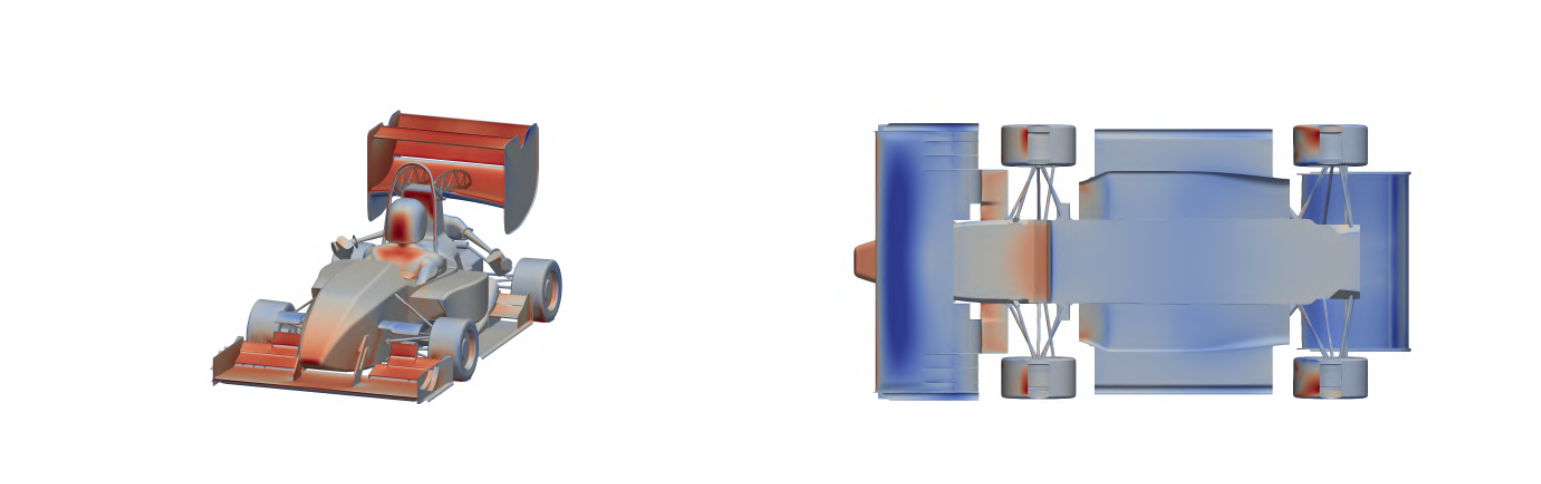
\includegraphics[width=\linewidth]{CP_MB_FLUENT}
		\end{subfigure}
		\par\vspace{0.2cm}
		\begin{subfigure}{0.48\linewidth}
			\centering
			
\includegraphics[width=\linewidth]{Report (2)/HY_MB_OF/Cp_car_iso.png}
		\end{subfigure}
		\hfill
		\begin{subfigure}{0.48\linewidth}
			\centering
			
\includegraphics[width=\linewidth]{Report/HY_MB_OF/Cè_car_bottom.png}
		\end{subfigure}
		\par\vspace{0.2cm}
		\begin{subfigure}{\linewidth}
			\centering
			
\includegraphics[width=\linewidth]{Report (2)/S284OF/Colorbarcp.png}
		\end{subfigure}
		\caption{Pressure coefficient distributions on the HY 2025 prototype, highlighting good correlation between Fluent (Top two images) and OpenFOAM (bottom two images).}
		\label{fig:cp_distrib}
	\end{figure}
	
	\begin{figure}[H]
		\begin{subfigure}{\linewidth}
			\centering
			
\includegraphics[width=\linewidth]{Report (2)/HY_MB_OF/U_0.4.png}
		\end{subfigure}        
		\par\vspace{0.2cm}
		\begin{subfigure}{\linewidth}
			\centering
			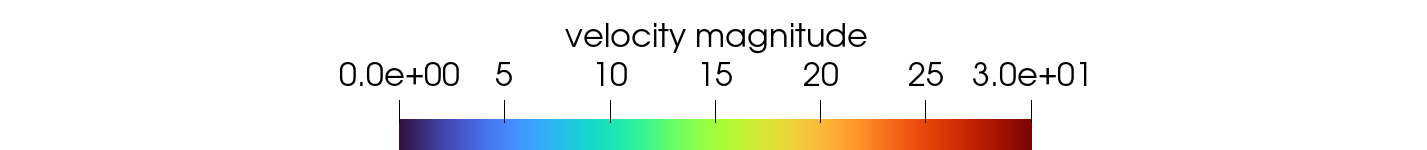
\includegraphics[width=\linewidth]{ColorbarU.png}
		\end{subfigure}
		\caption{Velocity magnitude gradient simulated with OpenFOAM. Unfortunately, it was not possible to procure the matching image from Fluent.}
		\label{fig:vel_mag_gradient}
	\end{figure}
	
	These results are physically realistic: velocity gradients, pressure gradients, and slipstream are consistent. It was not possible to provide post-processing pictures of this same simulation other than those found in Marco Bellucci's thesis \cite{Bellucci}.
	
	\begin{table}[htbp]
		\centering
		\renewcommand{\arraystretch}{1.3}
		\caption{Comparison of Fluent and OpenFOAM results using the same mesh}
		\label{tab:coefficienti2}
		\begin{tabular}{lcccc}
			\toprule
			\textbf{Tested Model} & Downforce & Drag & $C_LA$ & $C_DA$\\
			\midrule
			Fluent SST $k-\omega$                 & 259.5 N  & 114.6 N & 1.749 $m^2$ &0.773 $m^2$\\
			New mesh OpenFOAM {kOmegaSST}  & 258.9 N  & 114.4 N & 1.746 $m^2$&0.771$m^2$\\
			\bottomrule
		\end{tabular}
	\end{table}
	
	$$\varepsilon_{Df}= \frac{259.5-258.9}{259.5}\cdot 100\%= 0.23\%$$
	$$\varepsilon_{Dr}= \frac{114.6-114.4}{114.6}\cdot 100\%= 0.17\%$$
	This difference is negligible.
	
	\subsection{Results on the electric vehicle (2026)}
	\begin{figure}[H]
		\begin{subfigure}{0.48\linewidth}
			\centering
			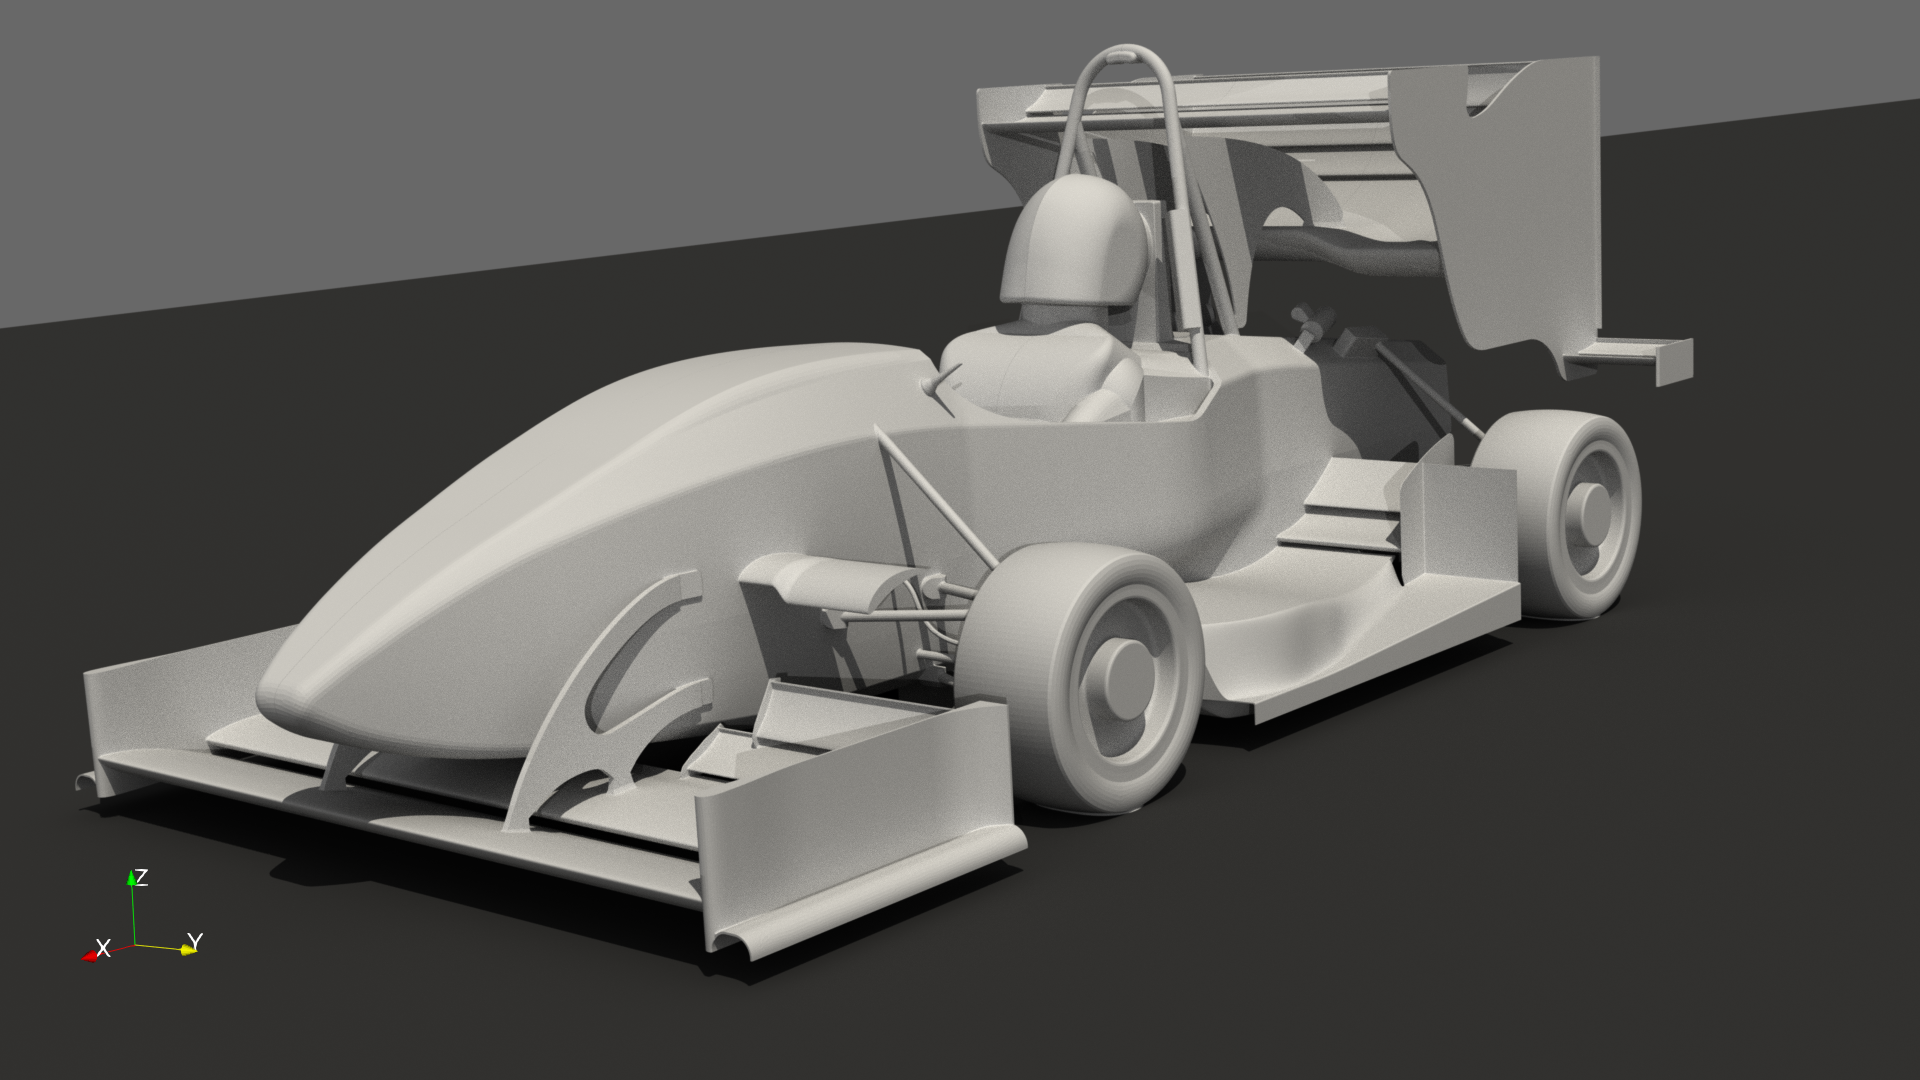
\includegraphics[width=\linewidth]{EV26.png}
		\end{subfigure}
		\hfill
		\begin{subfigure}{0.48\linewidth}
			\centering
			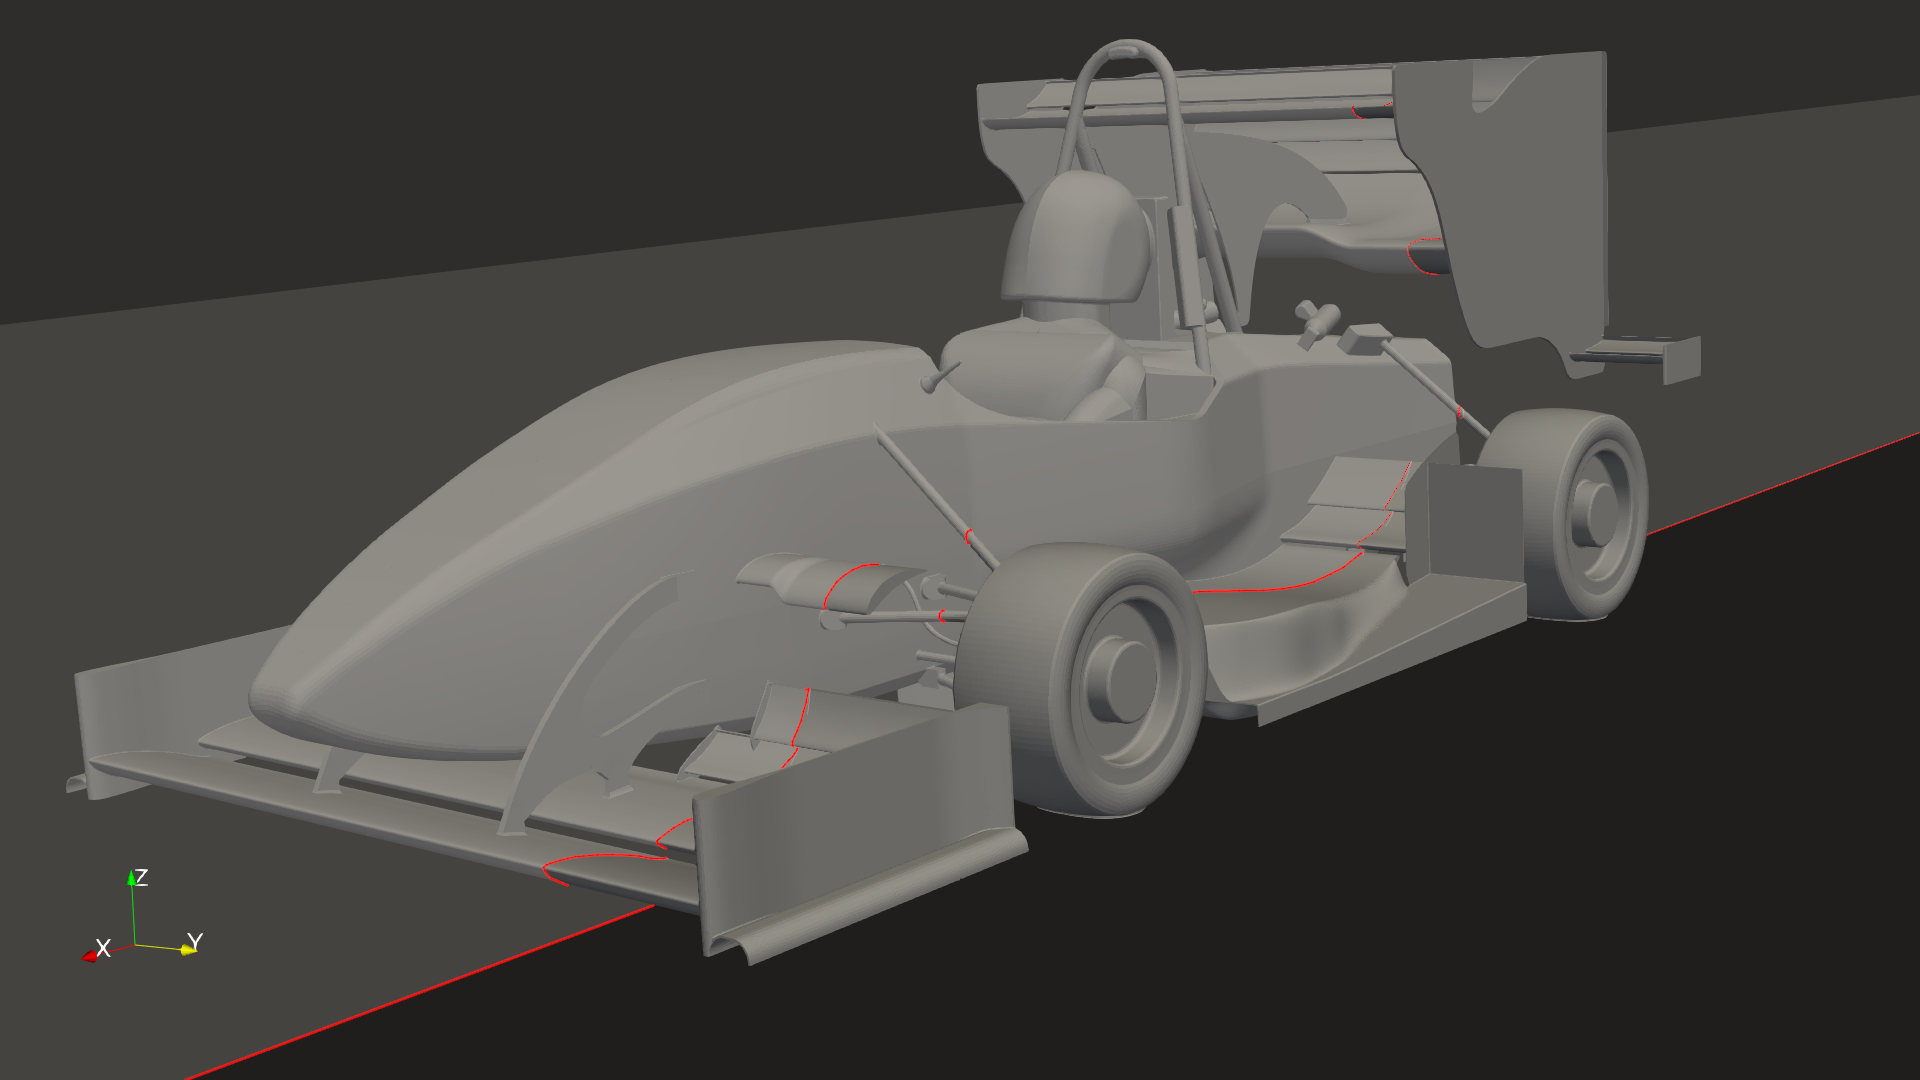
\includegraphics[width=\linewidth]{EV26_0.4.png}
		\end{subfigure}
		\caption{The EV26 car (Visione) in high quality on the left, and the plane we are evaluating at 0.4m from the center line on the right.}
		\label{fig:ev26_plane}
	\end{figure}
	
	Running the same mesh in both Fluent and OpenFOAM, I decided to focus my analysis on result quality and consistency, evaluating it from numerical values (Table \ref{tab:coefficienti3}) as well as color gradients all around the car. I have chosen to report only the values on a y-normal plane at 0.4 m (Figure \ref{fig:ev26_plane}) from the center line of the car, as this section features all the aerodynamic devices we installed on the car and shows the greatest discrepancies between the two simulations.
	I focused on pressure coefficient, velocity magnitude, and total pressure to visualize the flow field around the car.
	
	\begin{figure}[H]
		\begin{subfigure}{\linewidth}
			\centering
			
\includegraphics[width=\linewidth]{Immagini/Cp_0.4F.png}
		\end{subfigure}
		\par\vspace{0.2cm}
		\begin{subfigure}{\linewidth}
			\centering
			
\includegraphics[width=\linewidth]{Report (2)/S284OF/Cp_0.4.png}
		\end{subfigure}
		\caption{$C_{p}$ comparison between OpenFOAM (bottom) and Fluent (top).}
		\label{fig:cp_comp_front}
	\end{figure}
	
	\begin{figure}[H]
		\begin{subfigure}{\linewidth}
			\centering
			
\includegraphics[width=\linewidth]{Report (2)/S284OF/Plots_cp.png}
		\end{subfigure}
		\caption{Difference in the $C_p$ at the rear of the car between OpenFOAM (blue) and Fluent (red).}
		\label{fig:cp_diff_rear}
	\end{figure}
	
	A detailed comparative analysis between Fluent and OpenFOAM reveals a strong correlation at the front axle (Figure \ref{fig:cp_comp_front}). However, a localized divergence in the $C_p$ distribution (Figure \ref{fig:cp_diff_rear}), velocity magnitude (Figure \ref{fig:vel_mag_comp}), and total pressure is evident at the rear of the vehicle. This discrepancy is likely attributable to differing boundary condition implementations for the radiator porous media. Further investigation and rigorous alignment of the thermal-fluid boundary parameters are required to perfectly match the two solvers.
	
	\begin{figure}[H]
		\begin{subfigure}{\linewidth}
			\centering
			
\includegraphics[width=\linewidth]{Immagini/U_0.4F.png}
		\end{subfigure}
		\par\vspace{0.2cm}
		\begin{subfigure}{\linewidth}
			\centering
			
\includegraphics[width=\linewidth]{Report (2)/S284OF/U_0.4.png}
		\end{subfigure}
		\caption{Velocity magnitude comparison between OpenFOAM (bottom) and Fluent (top): We can clearly see a big difference at the rear of the car.}
		\label{fig:vel_mag_comp}
	\end{figure}
	
	
	\begin{table}[htbp]
		\centering
		\renewcommand{\arraystretch}{1.3}
		\caption{Comparison of Fluent and OpenFOAM results (EV 2026 prototype)}
		\label{tab:coefficienti3}
		\begin{tabular}{lcccc}
			\toprule
			\textbf{Tested Model} & Downforce & Drag &$C_LA$&$C_DA$\\
			\midrule
			Fluent SST $k-\omega$                 & 334.2 N & 132.6 N&$2.253m^2$& 0.894$m^2$\\
			New mesh OpenFOAM {kOmegaSST}  & 333.6 N  & 133.1 N &2.249$m^2$&0.897$m^2$\\
			\bottomrule
		\end{tabular}
	\end{table}
	
	\subsection{Design of Experiments}
	
	To further optimize the front wing performance, a parametric study focusing on multi-element "flags" (Figure \ref{fig:renault_flags}) has been structured. The purpose of these winglets is to condition the front tire wake, driving turbulent structures away from the underbody. The proposed Design of Experiments (DoE) matrix (Table \ref{tab:doe_flags}) will systematically evaluate the impact of their placement, spacing, and angle of attack on the global aerodynamic balance.
	
	\begin{figure}[H]
		\centering
		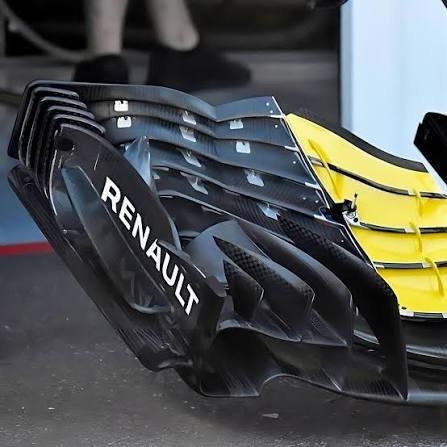
\includegraphics[width=0.7\linewidth]{RenaultF12018FW_Flags}
		\caption{An example of a 2018 F1 front wing by Renault F1 with clearly visible flags.}
		\label{fig:renault_flags}
	\end{figure}
	
	Initial simulations are planned to establish a baseline working design, followed by a detailed subdivision of parametric tests focusing on the number of flags, spatial coordinates (x and y positions), and angles of attack.
	
	\begin{table}[htbp]
		\centering
		\renewcommand{\arraystretch}{1.3}
		\caption{Design of Experiments configuration parameters (EV 2026 prototype)}
		\label{tab:doe_flags}
		\begin{tabular}{lccc}
			\toprule
			\textbf{Feature} & Test 1 & Test 2 & Test 3 \\
			\midrule
			x coordinate                 & 2.1m & 2.25m & 2.4m \\
			Number                 & 1 & 2 & 3 \\
			Spacing                 & 1* & 2* & 3* \\
			Angle of attack         & converging & parallel & diverging\\
			\bottomrule
		\end{tabular}
	\end{table}
	
	\section{Conclusion}
	As the primary objective of this internship was personal technical development, I consider the goal successfully achieved.
	I have developed a profound understanding of mesh quality requirements and their critical impact on CFD simulation accuracy.
	While the learning curve for OpenFOAM remains steep, I have mastered the fundamental principles of CFD, developed a steady-state RANS simulation equivalent to team standards, attained proficiency in ParaView for post-processing, and acquired essential Linux command-line skills.
	The following section provides a summarized workflow for executing simulations correctly:
	
	\bibliographystyle{ieeetr} 
	\bibliography{library}  
	
	
	% --- INIZIO APPENDICI ---
	\appendix
	\newpage
	\section{OpenFOAM Basic Tutorial}
	\begin{enumerate}
		\item Once the geometry is correctly configured in ANSA, open the Batch Mesh tool.
		Ensure the "Quality Criteria" column, typically set to \textit{Fluent Strict}, is updated.
		Modify each row to \textit{OpenFOAM Strict} by manual entry or bulk assignment.
		\item Execute the Batch Mesh process. During validation, verify that Quality Criteria are set to \textit{OpenFOAM Strict} and \textit{OpenFOAM Strict Conv2Poly}.
		\item Mesh validity is ensured if non-orthogonality remains below 70. Any cells exceeding this threshold require manual node adjustment. OpenFOAM \texttt{checkMesh} (already performed by the \texttt{Allrun} script) will provide information about the quality of the mesh. The expected output is \texttt{Mesh OK.}
		\item Export the mesh for OpenFOAM to a directory outside the simulation case folder.
		\item The standard case structure is as follows: 
		\begin{verbatim}
			case/
			|-- 0/
			|   |-- k
			|   |-- nut
			|   |-- omega
			|   |-- p
			|   `-- U
			|-- constant/
			|   |-- polyMesh/
			|   |-- physicalProperties
			|   `-- momentumTransport
			|-- system/
			|   |-- controlDict
			|   |-- fvSchemes
			|   |-- fvSolution
			|   `-- ...
			|-- Allrun
			`-- Allclean
			
		\end{verbatim}
		\item Copy the \texttt{polyMesh} folder into the \texttt{constant} directory, overwriting any existing versions.
		\item If new patches are introduced, they must be added to the \texttt{k, nut, omega, p, U} files and the \texttt{controlDict} to ensure accurate force calculations.
		\item Open the terminal and navigate to the case directory using \texttt{cd \$FOAM\_RUN/nameOfCase}.
		Execute the simulation using the provided script (\texttt{./Allrun}) or enter commands manually.
		\item Once the simulation is finished, the folder structure will look like this:
		\begin{verbatim}
			case/
			|-- 0/
			|   |-- k
			|   |-- nut
			|   |-- omega
			|   |-- p
			|   `-- U
			|-- {saved iterations}/
			|   |-- k
			|   |-- nut
			|   |-- omega
			|   |-- p
			|   `-- U
			|-- constant/
			|   |-- polyMesh/
			|   |-- physicalProperties
			|   `-- momentumTransport
			|-- system/
			|   |-- controlDict
			|   |-- fvSchemes
			|   |-- fvSolution
			|   `-- ...
			|--processor*/
			|   |-- {number of last saved iteration}/
			|   |   |-- k
			|   |   |-- nut
			|   |   |-- omega
			|   |   |-- p
			|   |   `-- U
			|--postProcessing
			|   |--forces_{FW/RW/Undertray/total}/
			|   |   |-- 0/
			|   |   |   |-- force.dat
			|   |   |   `-- moment.dat
			|   |   |-- {last iteration}/
			|   |   |   |-- force.dat
			|   |   |   `-- moment.dat
			|-- Allrun
			`-- Allclean
			
		\end{verbatim}
		\item Upon completion, launch ParaView via \texttt{paraFoam} or create a dummy file with \texttt{touch case.foam} and open it manually in ParaView.
		
	\end{enumerate}
	\newpage
	
	\begin{lstlisting}[style=bashStyle, caption={Script Allrun}]
		#!/bin/sh
		cd "${0%/*}" || exit 1
		
		# Load standard OpenFOAM functions
		. $WM_PROJECT_DIR/bin/tools/RunFunctions
		
		# 1. CLEANUP (Essential to prevent "file p not found" errors)
		echo "Cleaning processor directories..."
		rm -rf processor*
		rm -f log.*
		
		# 1. Mesh Validation
		echo "Validating mesh (checkMesh)..."
		checkMesh > log.checkMesh 2>&1
		# Extract and display results to terminal
		grep -iE "fail|error|ok" log.checkMesh | tail -n 1
		
		# 2. Initialization (Serial)
		echo "Initializing with potentialFoam..."
		# Force writing of p and U files
		potentialFoam -writePhi -writeU > log.potentialFoam 2>&1
		
		
		# 3. Decomposition (Must follow 0/ directory setup)
		echo "Decomposing mesh for 16 cores..."
		
		decomposePar -force > log.decomposePar 2>&1
		decomposePar -fields
		# 4. Mesh Optimization (Parallel)
		echo "Optimizing mesh (renumberMesh)..."
		mpirun -np 16 renumberMesh -overwrite -parallel > log.renumberMesh 2>&1
		
		# 5. Simulation Execution with Live Monitoring
		echo "Launching simulation (16 cores)..."
		echo "Monitoring residuals (U, p, omega, k):"
		echo "--------------------------------------------------------------------"
		
		# Use 'tee' for simultaneous logging and terminal output
		mpirun -np 16 --use-hwthread-cpus simpleFoam -parallel > log.simpleFoam 2>&1
		
		# 6. Final Reconstruction
		echo "--------------------------------------------------------------------"
		echo "Simulation complete. Reconstructing results..."
		reconstructPar -latestTime > log.reconstructPar 2>&1
		
		echo "Calculating Cp, Total Pressure, and Vorticity..."
		# Execute functionObjects defined in controlDict in serial mode
		postProcess -solver incompressibleFluid -latestTime
		
		echo "Post-processing complete. Open case using paraFoam."
	\end{lstlisting}
	
\end{document}